
\section{Independent platform for HW/SW Co-design}

%%%%%%% Insert Tanner Graph diagram and its explanation
\subsection{Raspberry Pi and DE0 Nano}

\begin{frame}
\frametitle{Raspberry Pi Features}   % Insert frame title between curly braces
\begin{itemize}
\item Its is an ARM based CPU capable of running real time operating systems
\item Sufficiently large number of GPIO pins available for external world application interfacing
\item Ethernet port on-board makes it easily accessible remotely
\item Easy to use USB port and Ethernet port helps configuring FPGA other development platform easy
\item On-broad JTAG port shall prove of great usage for co-design application debugging.
\end{itemize} 
\end{frame}



\begin{frame}
\frametitle{DE0-Nano Features}   % Insert frame title between curly braces
\begin{itemize}
\item Cyclone IV E family device EP4CE22F17C6 FPGA available on board having with 22,320 Logic Elements and 22,320 Logic Registers
\item Access to 72 GPIO pins and on-board ADC
\item Easy to configure and in system programming capability
\end{itemize} 
\end{frame}


\subsection{FPGA/CPLD Configuration using urJTAG}
\begin{frame}
\frametitle{FPGA/CPLD Configuration}   % Insert frame title between curly braces
\begin{itemize}
\item Raspberry Pi USB port and Ethernet port can be used for remote/hands-on FPGA/CPLD configuration
\item Raspberry Pi has on board JTAG port which can be used for JTAG debugging (JTAG port details not shared in Raspberry Pi documentation)
\item Easy OpenOCD installation help design and develop open-source hardware
\item Remote hardware upgrade of user application useful for hardware software co-design
\end{itemize} 
\end{frame}

\begin{frame}
\frametitle{FPGA/CPLD Configuration}   % Insert frame title between curly braces
The Figure below show a test set-up of implementation of Bezier interpolation.
   \begin{center}
   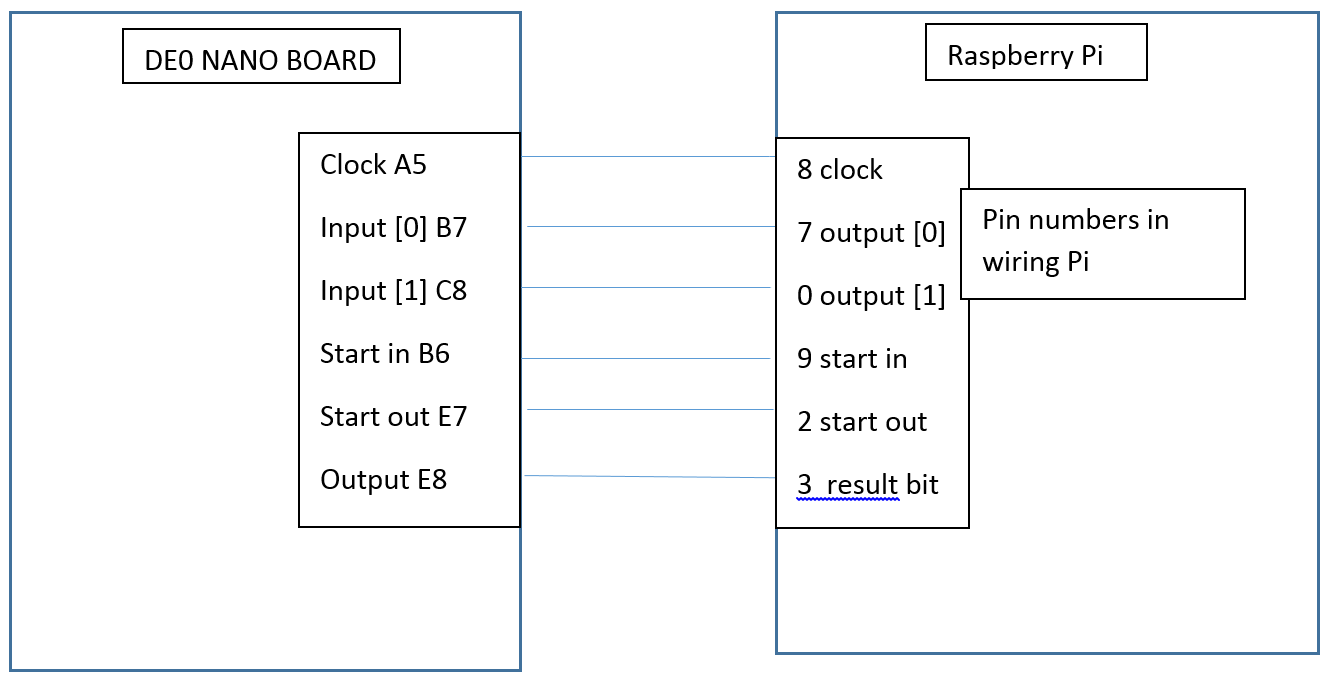
\includegraphics[scale=0.2]{./figs/DeNano_rPi}
   \end{center}
\tiny
Preformed by Siddharth and Abhinav, summer interns 2015, IIT Bombay.
\end{frame}